
\section{Method Overview}

\subsection{Foundation: Kimi K2 Base Model}

The foundation of Kimi K2.5 is Kimi K2~\citep{team2025kimik2}, a trillion-parameter mixture-of-experts (MoE) transformer~\citep{transformer} model pre-trained on 15 trillion high-quality text tokens. Kimi K2 employs the token-efficient MuonClip optimizer~\citep{jordan2024muon,liu2025muon} with QK-Clip for training stability. The model comprises 1.04 trillion total parameters with 32 billion activated parameters, utilizing 384 experts with 8 activated per token (sparsity of 48). For detailed descriptions of MuonClip, architecture design, and training infrastructure, we refer to the Kimi K2 technical report~\citep{team2025kimik2}.

\subsection{Model Architecture}



The multimodal architecture of Kimi K2.5 consists of three components: a three-dimensional native-resolution vision encoder (MoonViT-3D), an MLP projector, and the Kimi K2 MoE language model, following the design principles established in Kimi-VL~\citep{team2025kimivl}.

\paragraph{MoonViT-3D: Shared Embedding Space for Images and Videos}

In Kimi-VL, we employ MoonViT to natively process images at their original resolutions, eliminating the need for complex sub-image splitting and splicing operations. Initialized from SigLIP-SO-400M~\citep{zhai2023sigmoidlosslanguageimage}, MoonViT incorporates the patch packing strategy from NaViT~\citep{dehghani2023patchnpacknavit}, where single images are divided into patches, flattened, and sequentially concatenated into 1D sequences, thereby enabling efficient simultaneous training on images at varying resolutions.

To maximize the transfer of image understanding capabilities to video, we introduce \textbf{MoonViT-3D} with a unified architecture, fully shared parameters, and a consistent embedding space. By generalizing the ``patch n' pack`` philosophy to the temporal dimension, up to four consecutive frames are treated as a spatiotemporal volume: 2D patches from these frames are jointly flattened and packed into a single 1D sequence, allowing the identical attention mechanism to operate seamlessly across both space and time. While the extra temporal attention improves understanding on high-speed motions and visual effects, the sharing maximizes knowledge generalization from static images to dynamic videos, achieving strong video understanding performance (see in Tab.~\ref{tab:instruct_eval}) without requiring specialized video modules or architectural bifurcation. Prior to the MLP projector, lightweight temporal pooling aggregates patches within each temporal chunk, yielding $4\times$ temporal compression to significantly extend feasible video length. The result is a unified pipeline where knowledge and ability obtained from image pretraining transfers holistically to videos through one shared parameter space and feature representation.













\subsection{Pre-training Pipeline}

As illustrated in Table~\ref{tab:pretrainingdatavolume}, Kimi K2.5's pre-training builds upon the Kimi K2 language model checkpoint and processes approximately 15T tokens across three stages: first, standalone ViT training to establish a robust native-resolution visual encoder; second, joint pre-training to simultaneously enhance language and multimodal capabilities; and third, mid-training on high-quality data and long-context activation to refine capabilities and extend context windows.




\begin{table}[t]
\centering
\caption{Overview of training stages: data composition, token volumes, sequence lengths, and trainable components.}
\vspace{0.3em}
\renewcommand{\arraystretch}{1.2} % 稍微增加行间距，防止文字太挤
\begin{tabular}{lccc}
\toprule
\textbf{Stages} & \textbf{ViT Training} & \textbf{Joint Pre-training} & \textbf{Joint Long-context Mid-training} \\
\midrule
\textbf{Data} & 
\makecell[c]{Alt text \\ Synthesis Caption \\ Grounding, OCR, Video} & % 第1列：3行
\makecell[c]{+ \\ Text, Knowledge \\ Interleaving \\ Video, OS Screenshot} & % 第2列：4行
\makecell[c]{+ \\ High-quality Text \& Multimodal \\ Long Text, Long Video \\ Reasoning, Long-CoT } \\ % 第3列：5行
\midrule
\textbf{Sequence length} & 4096 & 4096 & 32768$\rightarrow$262144 \\
\midrule
\textbf{Tokens} & 1T & 15T & 500B$\rightarrow$200B \\
\midrule
\textbf{Training} & ViT & ViT \& LLM & ViT \& LLM \\
\bottomrule
\end{tabular}
\label{tab:pretrainingdatavolume}
\end{table}
\paragraph{ViT Training Stage}
The MoonViT-3D is continual pre-trained from SigLIP~\cite{zhai2023sigmoidlosslanguageimage} on image-text and video-text pairs, where the text components consist of a variety of targets: image alt texts, synthetic captions of images and videos, grounding bboxes, and OCR texts. Unlike the implementation in Kimi-VL~\cite{team2025kimivl}, this continual pre-training does not include a contrastive loss, but incorporates solely cross-entropy loss ${L}_{caption}$ for caption generation conditioned on input images and videos. We adopt a two-stage alignment strategy. In the first stage, we update the MoonViT-3D to align it with Moonlight-16B-A3B~\citep{liu2025muon} via the caption loss, consuming about 1T tokens with very few training FLOPs. This stage allows MoonViT-3D to primarily understand high-resolution images and videos. A very short second stage follows, updating only the MLP projector to bridge the ViT with the 1T LLM for smoother joint pre-training.

\paragraph{Joint Training Stages}
The joint pre-training stage continues from a near-end Kimi K2 checkpoint over additional 15T vision-text tokens at 4K sequence length. The data recipe extends Kimi K2's pre-training distribution by introducing unique tokens, adjusting data proportions with increased weight on coding-related content, and controlling maximum epochs per data source. The third stage performs long-context activation with integrated higher-quality mid-training data, sequentially extending context length via YaRN~\citep{peng2023yarn} interpolation. This yields significant generalization improvements in long-context text understanding and long video comprehension.



\subsection{Post-Training}
\subsubsection{Supervised Fine-Tuning}

Following the SFT pipeline established by Kimi K2 \citep{team2025kimik2}, we developed K2.5 by synthesizing high-quality candidate responses from K2, K2 Thinking and a suite of proprietary in-house expert models. Our data generation strategy employs specialized pipelines tailored to specific domains, integrating human annotation with advanced prompt engineering and multi-stage verification. 
This methodology produced a large-scale instruction-tuning dataset featuring diverse prompts and intricate reasoning trajectories, ultimately training the model to prioritize interactive reasoning and precise tool-calling for complex, real-world applications.




\subsubsection{Reinforcement Learning}
Reinforcement learning constitutes a crucial phase of our post-training. 
To facilitate joint optimization across text and vision modalities, as well as to enable PARL for agent swarm, we develop a Unified Agentic Reinforcement Learning Environment (Appendix~\ref{app:rl_infra}) and optimize the RL algorithms. 
Both text-vision joint RL and PARL are built upon the algorithms described in this section.
\paragraph{Policy Optimization}
For each problem $x$ sampled from a dataset $\mathcal{D}$, $K$ responses $\{y_1,\dots,y_K\}$ are generated using the previous policy $\pi_{\mathrm{old}}$.
We optimize the model $\pi_\theta$ with respect to the following objective: 
\begin{align}
L_{\mathrm{RL}}(\theta) = \mathbb{E}_{x \sim\mathcal{D}}
\left[ \frac{1}{N} \sum_{j=1}^K \sum_{i=1}^{|y_j|}
\mathrm{Clip}
\left(
\frac{\pi_{\theta}(y_j^i | x, y_j^{0:i})}{\pi_{\mathrm{old}}(y_j^i | x, y_j^{0:i}) }, \alpha, \beta
\right)
({r}(x, y_j) - \bar{r}(x))- \tau \left( \log \frac{\pi_{\theta}(y_j^i | x, y_j^{0:i})}{\pi_{\mathrm{old}}(y_j^i | x, y_j^{0:i}) } \right)^2
\right]
\, .
\label{eq:rl-objective}
\end{align}
Here $\alpha, \beta, \tau >0$ are hyperparameters, 
$y^j_{0:i}$ is the prefix up to the $i$-th token of the $j$-th response, 
$N=\sum_{i=1}^{K} |y_i|$ is the total number of generated tokens in a batch, 
$\bar{r}(x) = \frac{1}{K}\sum_{j=1}^K r(x, y_j)$ is the mean reward of all generated responses.   

This loss function departs from the policy optimization algorithm used in K1.5~\citep{team2025kimi} by introducing a token-level clipping mechanism designed to mitigate the off-policy divergence amplified by discrepancies between training and inference frameworks. 
The mechanism functions as a simple gradient masking scheme: policy gradients are computed normally for tokens with log-ratios within the interval $[\alpha, \beta]$, while gradients for tokens falling outside this range are zeroed out. 
Notably, a key distinction from standard PPO clipping \citep{schulman2017proximal} is that our method relies strictly on the log-ratio to explicitly bound off-policy drift, regardless of the sign of the advantages. 
This approach aligns with recent strategies proposed to stabilize large-scale RL training \citep{yao2025offpolicy, IcePop2025}. 
Empirically, we find this mechanism essential for maintaining training stability in complex domains requiring long-horizon, multi-step tool-use reasoning.
We employ the MuonClip optimizer~\citep{jordan2024muon,liu2025muon} to minimize this objective. 


\paragraph{Reward Function} 
We apply a rule-based outcome reward for tasks with verifiable solutions, such as reasoning and agentic tasks. 
To optimize resource consumption, we also incorporate a budget-control reward aimed at enhancing token efficiency. % (Section \ref{sec:te}). 
For general-purpose tasks, we employ Generative Reward Models (GRMs) that provide granular evaluations aligned with Kimi's internal value criteria. 
In addition, for visual tasks, we design task-specific reward functions to provide fine-grained supervision. 
For visual grounding and point localization tasks, we employ an F1-based reward with soft matching: grounding tasks derive soft matches from Intersection over Union (IoU) and point tasks derive soft matches from Gaussian-weighted distances under optimal matching. 
For polygon segmentation tasks, we rasterize the predicted polygon into a binary mask and compute the segmentation IoU against the ground-truth mask to assign the reward. 
For OCR tasks, we adopt normalized edit distance to quantify character-level alignment between predictions and ground-truth. 
For counting tasks, rewards are assigned based on the absolute difference between predictions and ground-truth. 
Furthermore, we synthesize complex visual puzzle problems and utilize an LLM verifier (Kimi K2) to provide feedback.


\paragraph{Generative Reward Models}
Kimi K2 leverages a self-critique rubric reward for open-ended generation \cite{team2025kimik2}, and K2.5 extends this line of work by systematically deploying \emph{Generative Reward Models (GRMs)} across a broad range of agentic behaviors and multimodal trajectories. Rather than limiting reward modeling to conversational outputs, we apply GRMs on top of verified reward signals in diverse environments, including chat assistants, coding agents, search agents, and artifact-generating agents. Notably, GRMs function not as binary adjudicators, but as fine-grained evaluators aligned with Kimi's values that are critical to user experiences, such as helpfulness, response readiness, contextual relevance, appropriate level of detail, aesthetic quality of generated artifacts, and strict instruction following. This design allows the reward signal to capture nuanced preference gradients that are difficult to encode with purely rule-based or task-specific verifiers.
To mitigate reward hacking and overfitting to a single preference signal, we employ multiple alternative GRM rubrics tailored to different task contexts.


\paragraph{Token Efficient Reinforcement Learning}
\label{sec:te}
Token efficiency is central to LLMs with test-time scaling. 
While test-time scaling inherently trades computation for reasoning quality, practical gains require algorithmic innovations that actively navigate this trade-off. 
Our previous findings indicate that imposing a problem-dependent budget effectively constrains inference-time compute, incentivizing the model to generate more concise chain of thought reasoning patterns without unnecessary token expansion \citep{team2025kimi,team2025kimik2}. 
However, we also observe a \emph{length-overfitting phenomenon}: models trained under rigid budget constraints often fail to generalize to higher compute scales. Consequently, they cannot effectively leverage additional inference-time tokens to solve complex problems, instead defaulting to truncated reasoning patterns.



To this end, we propose \emph{Toggle}, 
a training heuristic that alternates between {inference-time scaling} and {budget-constrained optimization}: 
for learning iteration $t$, 
the reward function is defined by 
\begin{align*}
\tilde{r}(x,y) = 
\begin{cases} 
r(x, y) \cdot \mathbb{I}\left\{ \frac{1}{K} \sum_{i=1}^K r(x, y_i)  < \lambda\ \mathrm{or}\ |y_i| \leq \mathrm{budget(x)} \right\} & \text{if } \lfloor t/m \rfloor \pmod 2 = 0\ (\mathrm{{Phase 0}}) \\
r(x, y) & \text{if } \lfloor t/m \rfloor \pmod 2 = 1\ (\mathrm{{Phase 1}}) 
\end{cases}
\, .
\end{align*}
where $\lambda$ and $m$ are hyper-parameters of the algorithm and $K$ is the number of rollouts per problem. 
Specifically, the algorithm alternates between two optimization phases every $m$ iterations:
\begin{itemize}

\item {Phase0} (\emph{budget limited phase}): 
The model is trained to solve the problem within a task-dependent token budget. 
To prevent a premature sacrifice of quality for efficiency, this constraint is conditionally applied: it is only enforced when the model's mean accuracy for a given problem exceeds the threshold $\lambda$.

\item {Phase1} (\emph{standard scaling phase}): The model generates responses up to the maximum token limit, encouraging the model to leverage computation for better inference-time scaling. 

\end{itemize}

The problem-dependent budget is estimated from the $\rho$-th percentile of token lengths among the subset of correct responses:
\begin{equation}
\mathrm{budget}(x) = \text{Percentile}\left(\{ |y_j| \mid r(x, y_i) = 1, i=1,\dots, K \}, \rho \right) \,.
\end{equation}
This budget is estimated once at the beginning of training and remains fixed thereafter. 
Notably, Toggle functions as a stochastic alternating optimization for a bi-objective problem. It is specifically designed to reconcile reasoning capabilities with computational efficiency. %In our experiments, we use $\lambda = 7/8$, $m=2$ and $\rho = 90\%$.


\begin{figure}[t]
    \centering
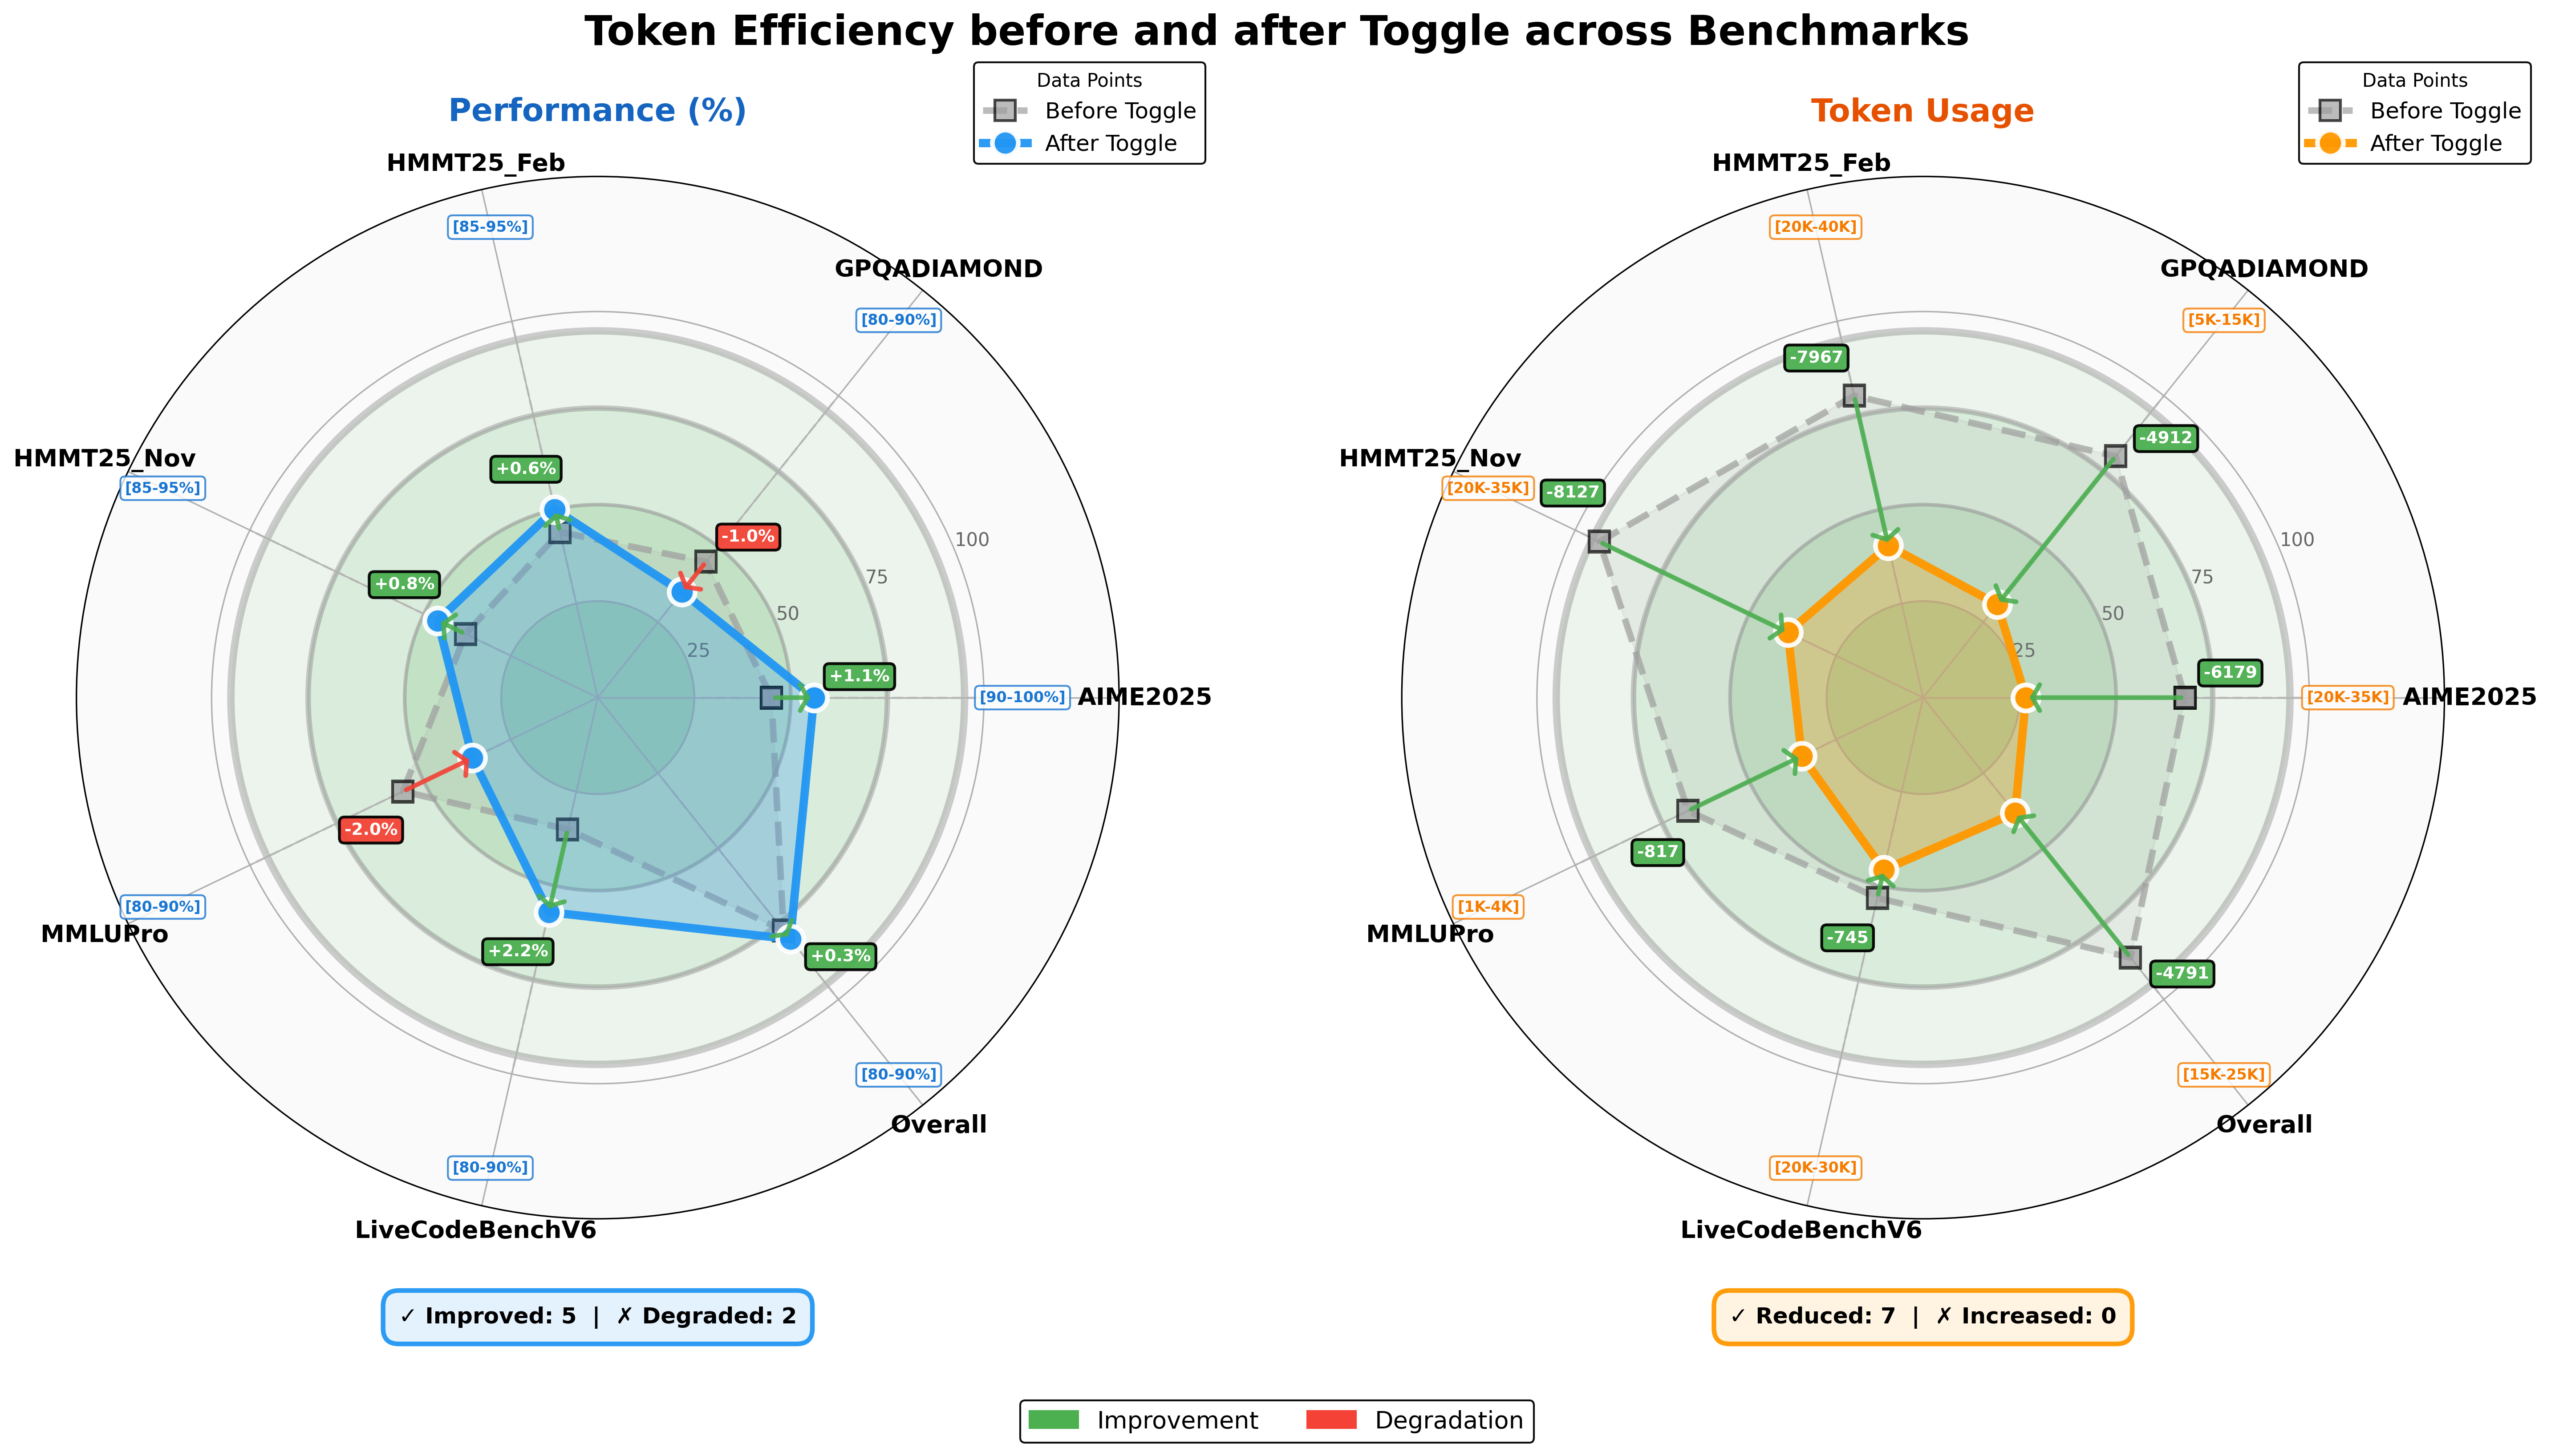
\includegraphics[width=0.8\linewidth, keepaspectratio]{figures/te-k2-thinking-radar.png}
    \caption{Comparison of model performance and token usage for Kimi K2 Thinking following token-efficient RL.}
    \label{fig:k25_performance}
\end{figure}

We evaluate the effectiveness of Toggle on K2 Thinking~\citep{moonshotai2025kimi}.
As shown in Figure~\ref{fig:k25_performance}, we observe a consistent reduction in output length across nearly all benchmarks.
On average, Toggle decreases output tokens by 25$\sim$30\% with a negligible impact on performance. 
We also observe that redundant patterns in the chain-of-thought, such as repeated verifications and mechanical calculations, decrease substantially.
Furthermore, Toggle shows strong domain generalization. 
For example, when trained exclusively on mathematics and programming tasks, the model still achieves consistent token reductions on GPQA and MMLU-Pro with only marginal degradation in performance (Figure \ref{fig:k25_performance}). 










 




\subsection{Training Infrastructure}

Kimi K2.5 inherits the training infrastructure from Kimi K2~\citep{team2025kimik2} with minimal modifications.  For multimodal training, we propose Decoupled Encoder Process, where the vision encoder is incorporated into the existing pipeline with negligible additional overhead.

\subsubsection{Decoupled Encoder Process (DEP)}

In a typical multimodal training paradigm utilizing Pipeline Parallelism (PP), the vision encoder and text embedding are co-located in the first stage of the pipeline (Stage-0). However, due to the inherent variations of multimodal input size (e.g., image counts and resolutions), Stage-0 suffers from drastic fluctuations in both computational load and memory usage. This forces existing solutions to adopt custom PP configurations for vision-language models --- for instance, \cite{team2025kimivl} manually adjusts the number of text decoder layers in Stage-0 to reserve memory. While this compromise alleviates memory pressure, it does not fundamentally resolve the load imbalance caused by multimodal input sizes. More critically, it precludes the direct reuse of parallel strategies that have been highly optimized for text-only training.

Leveraging the unique topological position of the visual encoder within the computation graph --- specifically, its role as the start of the forward pass and the end of the backward pass --- our training uses \textbf{Decoupled Encoder Process (DEP)}, which is composed of three stages in each training step:

\begin{itemize}
\item \textbf{Balanced Vision Forward:} We first execute the forward pass for all visual data in the global batch. Because the vision encoder is small, we replicate it on all GPUs regardless of other parallelism strategies. During this phase, the forward computational workload is evenly distributed across all GPUs based on load metrics (e.g., image or patch counts). This eliminates load-imbalance caused by PP and visual token counts. To minimize peak memory usage, we discard all intermediate activations, retaining only the final output activations. The results are gathered back to PP Stage-0;

\item \textbf{Backbone Training:} This phase performs the forward and backward passes for the main transformer backbone. By discarding intermediate activations in the preceding phase, we can now fully leverage any efficient parallel strategies validated in pure text training. After this phase, gradients are accumulated at the visual encoder output;
\item \textbf{Vision Recomputation \& Backward:} We re-compute the vision encoder forward pass, followed by a backward pass to compute gradients for parameters in the vision encoder;
\end{itemize}

DEP not only achieves load-balance, but also decouples the optimization strategy of the vision encoder and the main backbone. K2.5 seamlessly inherits the parallel strategy of K2, achieving a multimodal training efficiency of 90\% relative to text-only training. We note a concurrent work, LongCat-Flash-Omni~\citep{team2025longcat}, shares a similar design philosophy.



